\documentclass[]{article}
\usepackage{lmodern}
\usepackage{amssymb,amsmath}
\usepackage{ifxetex,ifluatex}
\usepackage{fixltx2e} % provides \textsubscript
\ifnum 0\ifxetex 1\fi\ifluatex 1\fi=0 % if pdftex
  \usepackage[T1]{fontenc}
  \usepackage[utf8]{inputenc}
\else % if luatex or xelatex
  \ifxetex
    \usepackage{mathspec}
  \else
    \usepackage{fontspec}
  \fi
  \defaultfontfeatures{Ligatures=TeX,Scale=MatchLowercase}
\fi
% use upquote if available, for straight quotes in verbatim environments
\IfFileExists{upquote.sty}{\usepackage{upquote}}{}
% use microtype if available
\IfFileExists{microtype.sty}{%
\usepackage{microtype}
\UseMicrotypeSet[protrusion]{basicmath} % disable protrusion for tt fonts
}{}
\usepackage[margin=1in]{geometry}
\usepackage{hyperref}
\hypersetup{unicode=true,
            pdftitle={Excercise 1},
            pdfauthor={Nam Tran},
            pdfborder={0 0 0},
            breaklinks=true}
\urlstyle{same}  % don't use monospace font for urls
\usepackage{graphicx,grffile}
\makeatletter
\def\maxwidth{\ifdim\Gin@nat@width>\linewidth\linewidth\else\Gin@nat@width\fi}
\def\maxheight{\ifdim\Gin@nat@height>\textheight\textheight\else\Gin@nat@height\fi}
\makeatother
% Scale images if necessary, so that they will not overflow the page
% margins by default, and it is still possible to overwrite the defaults
% using explicit options in \includegraphics[width, height, ...]{}
\setkeys{Gin}{width=\maxwidth,height=\maxheight,keepaspectratio}
\IfFileExists{parskip.sty}{%
\usepackage{parskip}
}{% else
\setlength{\parindent}{0pt}
\setlength{\parskip}{6pt plus 2pt minus 1pt}
}
\setlength{\emergencystretch}{3em}  % prevent overfull lines
\providecommand{\tightlist}{%
  \setlength{\itemsep}{0pt}\setlength{\parskip}{0pt}}
\setcounter{secnumdepth}{0}
% Redefines (sub)paragraphs to behave more like sections
\ifx\paragraph\undefined\else
\let\oldparagraph\paragraph
\renewcommand{\paragraph}[1]{\oldparagraph{#1}\mbox{}}
\fi
\ifx\subparagraph\undefined\else
\let\oldsubparagraph\subparagraph
\renewcommand{\subparagraph}[1]{\oldsubparagraph{#1}\mbox{}}
\fi

%%% Use protect on footnotes to avoid problems with footnotes in titles
\let\rmarkdownfootnote\footnote%
\def\footnote{\protect\rmarkdownfootnote}

%%% Change title format to be more compact
\usepackage{titling}

% Create subtitle command for use in maketitle
\newcommand{\subtitle}[1]{
  \posttitle{
    \begin{center}\large#1\end{center}
    }
}

\setlength{\droptitle}{-2em}

  \title{Excercise 1}
    \pretitle{\vspace{\droptitle}\centering\huge}
  \posttitle{\par}
    \author{Nam Tran}
    \preauthor{\centering\large\emph}
  \postauthor{\par}
    \date{}
    \predate{}\postdate{}
  

\begin{document}
\maketitle

\subsection{Part 1}\label{part-1}

In this part, I aimed to find a relationship that could dispel the
notion that green ratings equate to higher rents, and thus higher
revenues.I first started by grouping the buildings by whether or not
they attained a green rating. Here we see some quick differences in
rent, leasing rate etc.

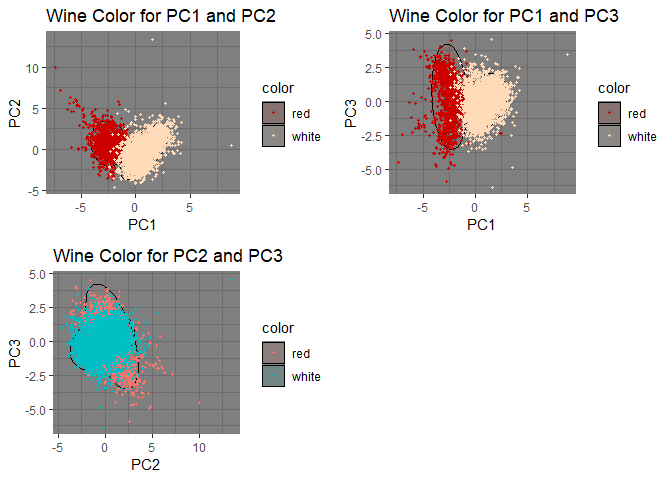
\includegraphics{Excercise1_raw_files/figure-latex/unnamed-chunk-1-1.pdf}

The pros of green buildings are evident here, but are the higher rents
due to green ratings or other variables? Next, I examined the
relationship between rent and age.

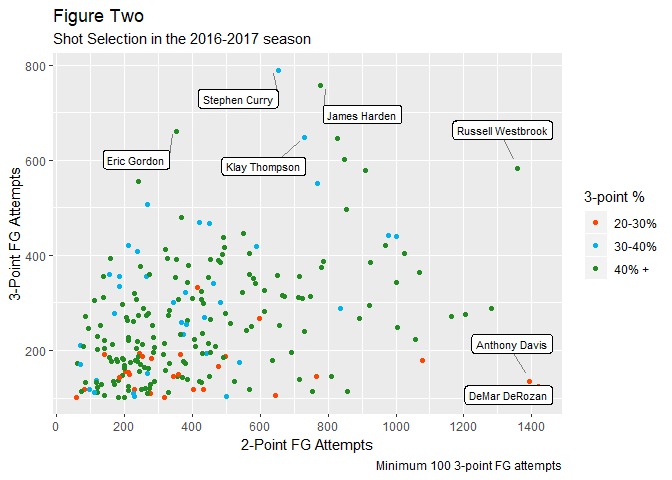
\includegraphics{Excercise1_raw_files/figure-latex/unnamed-chunk-2-1.pdf}
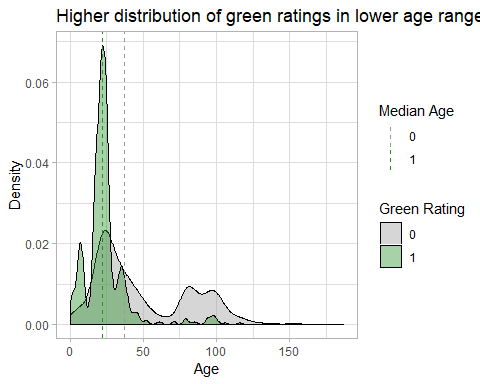
\includegraphics{Excercise1_raw_files/figure-latex/unnamed-chunk-2-2.pdf}

Here, it is clear that rent is lower in the newer buildings. I did this
by dividing the age into ten quantiles and finding the average rent in
each quantile. The age density graph serves to reinforce the notion that
green buildings are much newer than non-green buildings. This certainly
doesn't prove much, but it does make the ``data guru'''s assertions a
bit odd.

\subsection{Part 2}\label{part-2}

In this section, I mainly looked to answer two questions: What is the
best time of day to fly to minimize delays and What is the best time of
year to fly to minimize delays? Here are the results:
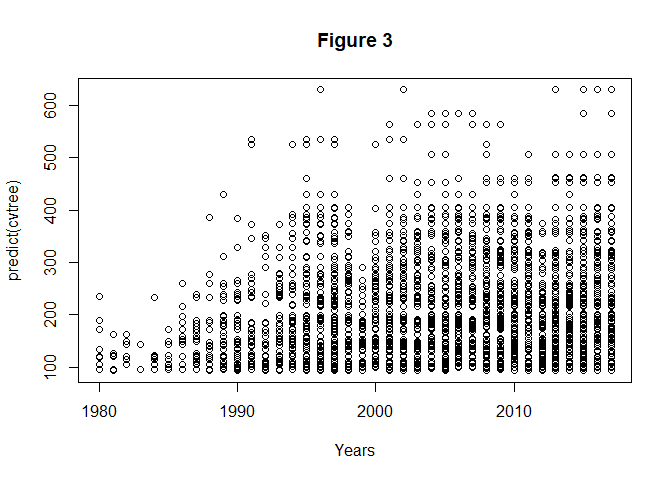
\includegraphics{Excercise1_raw_files/figure-latex/unnamed-chunk-3-1.pdf}

For the times of day, I divided the 24 hours into 4, 6 hour periods.
Early morning flights ran from 12 a.m. to 6 a.m., morning flights from
6.a.m. to 12 p.m. and onwards. Unsurprisingly, the least amount of
delays occured in the ``early morning'' time frame, and in fact, the
average flight was ahead of time! When looking at seasons, the results
are also rather unsurprisng.

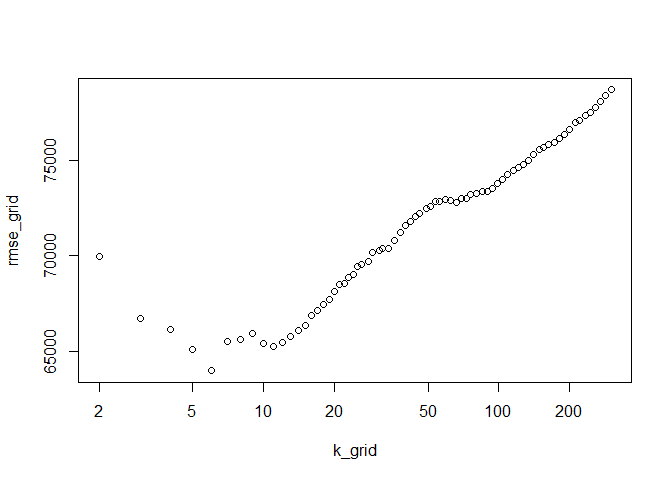
\includegraphics{Excercise1_raw_files/figure-latex/unnamed-chunk-4-1.pdf}
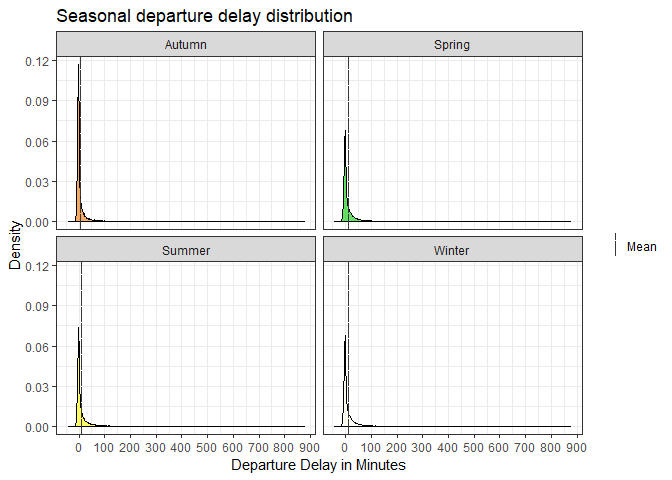
\includegraphics{Excercise1_raw_files/figure-latex/unnamed-chunk-4-2.pdf}

For the seasons, I divided the months by the traditional definitions.
Winter runs from December to february, Spring going from March to May,
Summer spanning June through August, and Autumn rounding it out from
September to November. These results follow traditional intuition.
Autumn doesn't span many major holidays, and it is also one of the more
fair weather seasons in this area. I quickly also looked at delay times
by destination. The only major surprise is the absurdly high delay time
from DSM which is Des Moines International Airport. Perhaps it is just a
victim of severe outliers due to extreme weather or other unlikely
delays.

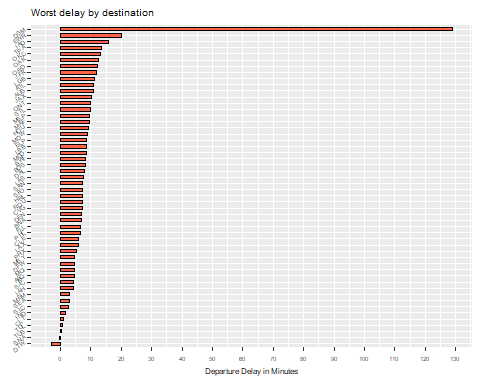
\includegraphics{Excercise1_raw_files/figure-latex/unnamed-chunk-5-1.pdf}

\subsection{Part 3}\label{part-3}

In this part, I begin by dividng the data by two specific trims, 350 and
65 AMG. Then after creating the training and testing splits, I use
K-nearest neighbors to build a model. I run each trim from K = 3 to K =
100, finding the out of sample rmse for each. I then used the minimum
rsme of the set to build the final predictive graph.

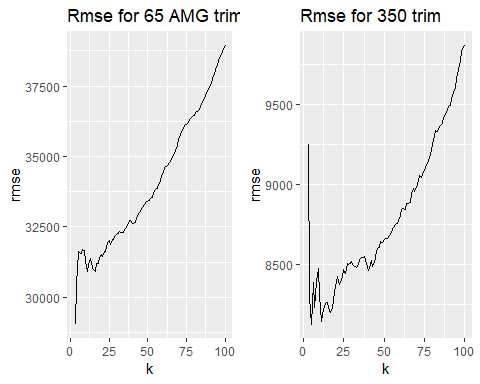
\includegraphics{Excercise1_raw_files/figure-latex/unnamed-chunk-6-1.pdf}

\begin{verbatim}
## Optimal K for 65 AMG trim:  20
\end{verbatim}

\begin{verbatim}
## Optimal K for 350 trim:  63
\end{verbatim}

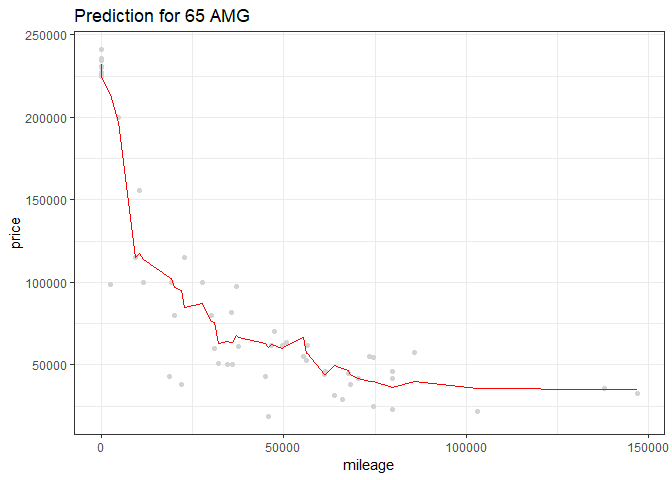
\includegraphics{Excercise1_raw_files/figure-latex/unnamed-chunk-6-2.pdf}
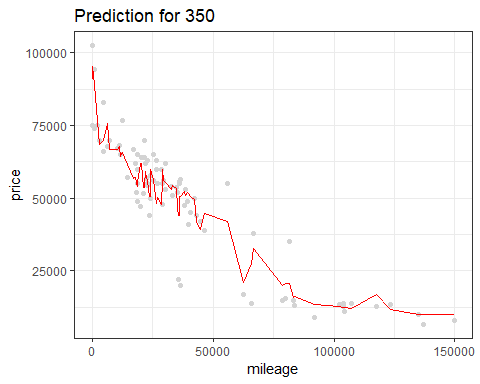
\includegraphics{Excercise1_raw_files/figure-latex/unnamed-chunk-6-3.pdf}

Overall, the 350 trim has a higher optimal K value. I think this is due
to the larger sample size available. It enables the model to ``explain''
more of the variance. However, with this training and test split, the
results do vary from run to run.


\end{document}
